\section{Minimax Algorithm} 
\label{sec:Minimax Algorithm}

\subsection{Introduction to Minimax}
\label{subsec:Introduction to Minimax}
The Minimax algorithm is a recursive algorithm which is used in turn-based games like chess and tic-tac-toe, 
to make the AI player consider all possible moves and choose the best one.

\subsection{Explanation of Minimax}
\label{subsec:Explanation of Minimax}
\subsubsection{About Minimax}
First, it is important to understand the meaning behind recursive code. 
When code is recursive, it simply means that you are writing a function that calls itself with updated arguments until it reaches some condition the function wants to return. 
In the Minimax algorithm we want to make the function call itself to keep looking at more possible future moves, 
and ultimately decide which move is the best move to make on the AI’s current board.
\subsubsection{Why is it called Minimax}
The idea behind minimax is that the algorithm expects the game to be a turn-based 2-player game, and the algorithm defines these 2 players as the minimizer and the maximizer. 
This simply means that the algorithm always expects the minimizer to pick the move with the lowest score, and the maximizer to do the opposite. 
Here is an example: Let us say the maximizer is the human player and the minimizer is the AI player in this scenario.\\

Look at this Tic-Tac-Toe board:\\
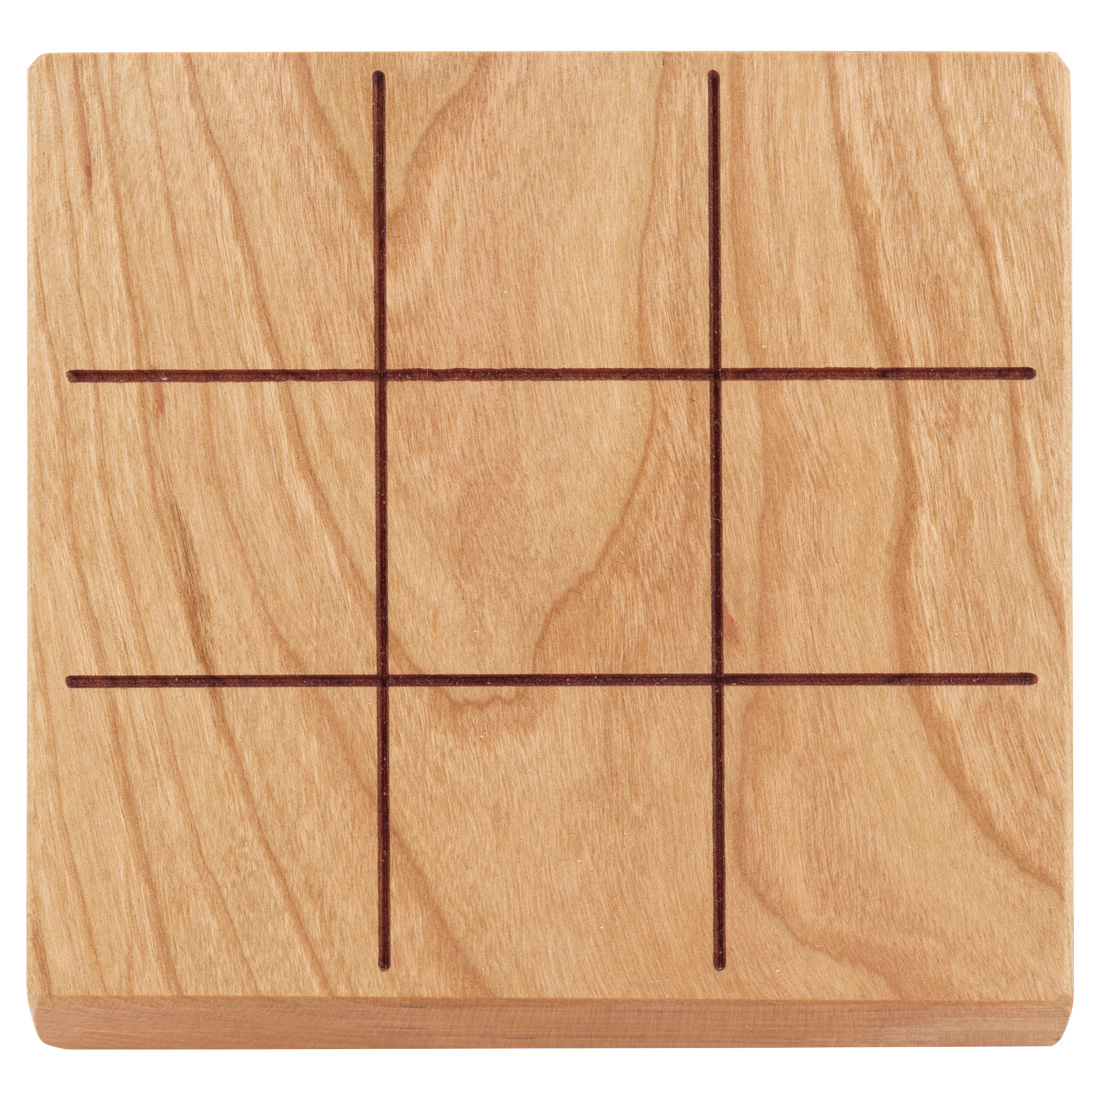
\includegraphics[width=\textwidth]{89-137-4480.jpg}\\
In this scenario the AI player goes first as “X” and tries to figure out the most rational move of the 9 moves possible. 
It does this by predicting what the opposing player, maximizer would then do on his next move and so on until it has found the fastest way to win for that one move. 
Basically, the algorithm runs a simulated game on each of the current board’s possible moves, against the maximizer, 
and when it is done with one move it backtracks back to the current board with that moves score value, to run a new simulation on the next move. 
When it has simulated how to win by all the possible moves it will then make the move that will help it win the fastest.\\

Let us see another example:\\
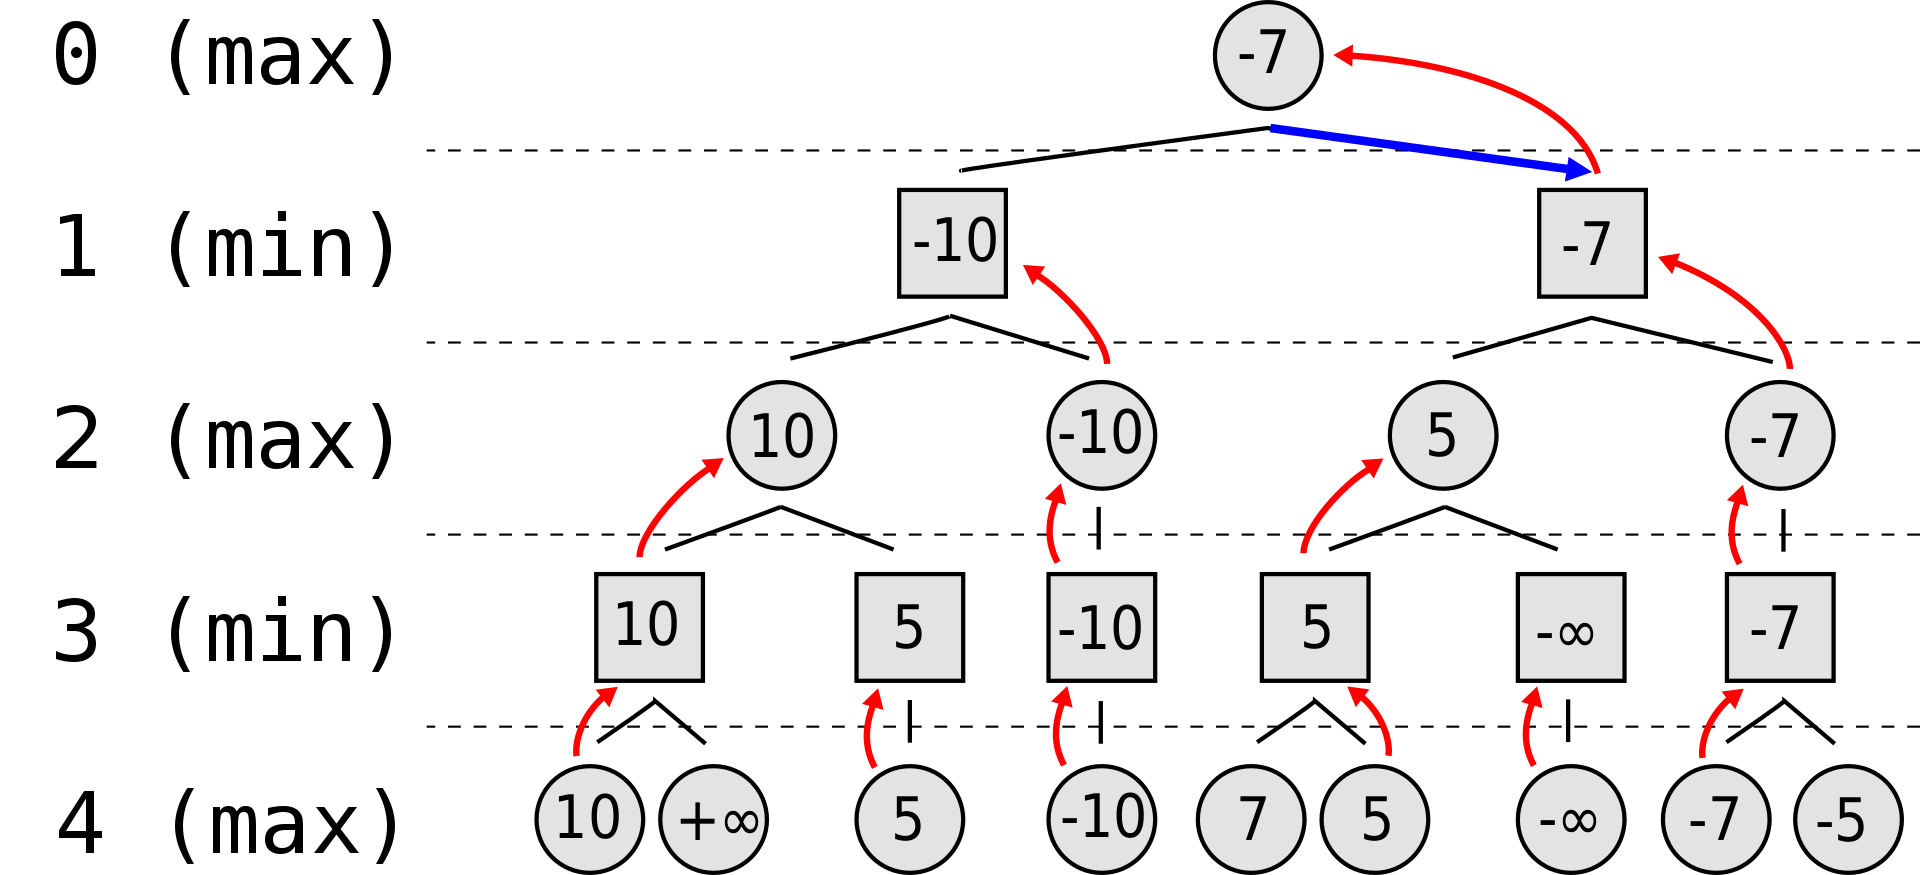
\includegraphics[width=\textwidth]{1920px-Minimax.svg.png}\\
If you look at the tree above it shows an example of how the minimax works. In this scenario the maximizer goes first, and he has 2 possible moves. 
He would therefore explore the first move first, marked -10. At this point the algorithm has not simulated this move yet and therefore does not know that value yet. 
So first he just tries the moves leftmost in the tree until he hits the depth 4 which is the bottom in this scenario. He would end up with a value of 10 which would be good for the maximizer. 
But we need to take the minimizer into account, so we backtrack once to see the other move which is +infinity, 
which we can say for sure the minimizer would never pick that route, which means we keep the score 10 in mind while we backtrack to the next point where the minimizer has a move. 
As is seen this route only gives both players one choice on each of their respective turns. 
The last move has a -10 score so we backtrack with that score once again and end up 10 and -10 on the 2 moves the minimizer can make. 
If the maximizer chooses this route the point value of the move would therefore be -10 as the minimizer always goes for the lesser score.\\
The algorithm then does the same thing for the other move and finds that this move will serve him better as it will yield -7 move value which is still bad for the maximizer but less bad then a -10 score.

\subsection{Implementation of Minimax}
\label{subsec:Implementation of Minimax}
% Show our own code!

\clearpage